\subsection{Opgave 26}

Tegn grafen for en funktion f, der opfylder følgende:
\begin{itemize}
    \item definitionsmængden er $Dm(f) = [-4;5]$
    \item funktionen har et maksimum i punktet (3;6)
\end{itemize}

\ans

Når definitionsmængden er i det lukkede interval [-4, 5] betyder det at vores funktion har to lukkede punkter
i x værdierne $x = -4$ of $x = 5$. Derudover får vi at vide at funktionen har et maksimum i punktet (3;6).
Det betyder at når funktionen f har x værdien $x = 3$ skal dens y værdi være 
$y = 6$ og på intet andet sted mellem $x = -4$ og $x = 5$ må funktionen f
have en y værdi der er større end eller lig med 6 ($y \geq 6$).
Til de 2 lukkede punkter kan vi altså vælge en hvilket som helst y værdi som er skarpt mindre end 6 ($y < 6$).
Jeg vælger $y = 1$ i begge lukkede punkter og tegner nu de 3 punkter ind i et koordinatsystem.
Forbinder man de 3 punkter med 2 rette linjer har vi nu tegnet en funktion som overholder kravene.

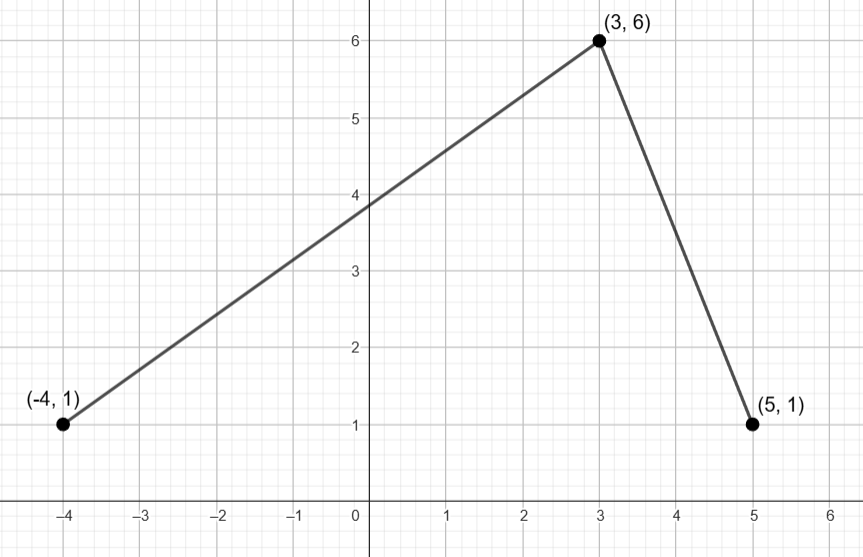
\includegraphics[width=10cm]{Opgave_21-30/Opgave_26/26.png}





